\documentclass[12pt,a4paper]{scrreprt}
\usepackage[utf8]{inputenc}
\usepackage[ngerman]{babel}
\usepackage{amsmath}
\usepackage{amsfonts}
\usepackage{amssymb}
\usepackage{todonotes}	
\usepackage[]{graphicx} 
\usepackage{hyperref}


\title{Handbuch \\ Gemeinsame, verteilte Überwachung eines Gebietes auf Eindringlinge}
\author{Dennis Lisiecki, Torsten Kühl}

\begin{document}

\maketitle	%Titelblatt erstellen
\tableofcontents	%Inhaltsverzeichnis erstellen


\chapter{Vorbereitung}
\section{Vorwort}
Im Folgendem stellen wir ein Handbuch zur Verfügung, um den Umgang mit dem Programm Codis zu zeigen. Codis steht kurz für \textit{Cooperative, Distributed Surveillance}. Codis realisiert eine kooperative, verteilte Überwachung eines Gebiets auf Eindringlinge, bei der mehrere Raspberry Pis, auf denen Codis gleichzeitig läuft, ein Gebiet aus mehreren Blickwinkeln überwachen. Der Ansatz der kooperativen, verteilten Überwachung soll Vorteile gegenüber nicht-verteilten Überwachungssystemen bieten. Vorteile sollen unter anderem sein, dass Codis eine bessere Ausfalltoleranz hat gegenüber nicht-verteilte Überwachungssysteme und eine verbesserte Genauigkeit beim Entdecken von Eindringlingen. Die folgenden Seiten zeigen Ihnen, woher Sie sich Codis holen und wie es verwendet wird. Wichtiger Hinweis: Codis ist zurzeit in einem Prototypen-Status und nicht für den Einsatz im Freien geeignet. Das liegt daran, weil Codis das UDP-Protokoll verwendet, um die Netzwerkkommunikation im Codis-System zu realisieren. Das UDP-Protokoll hat den Nachteil, dass Pakete eventuell nicht ankommen können. Dementsprechend können beim Betrieb von Codis Fehler auftreten. Außerdem wird eine Internet-Verbindung benötigt, um Nachrichten per UDP versenden zu können.

\section{Diese Teile werden für Codis benötigt}
\begin{itemize}
\item Raspberry Pi
\item Pi NoIR-Kamera
\item PIR-Sensor
\item Steckbrückenkabel um den PIR-Sensor mit dem Raspberry zu verbinden
\end{itemize}

\chapter{Aufbau}
\section{Die Kamera}
 \begin{figure}[h] \centering 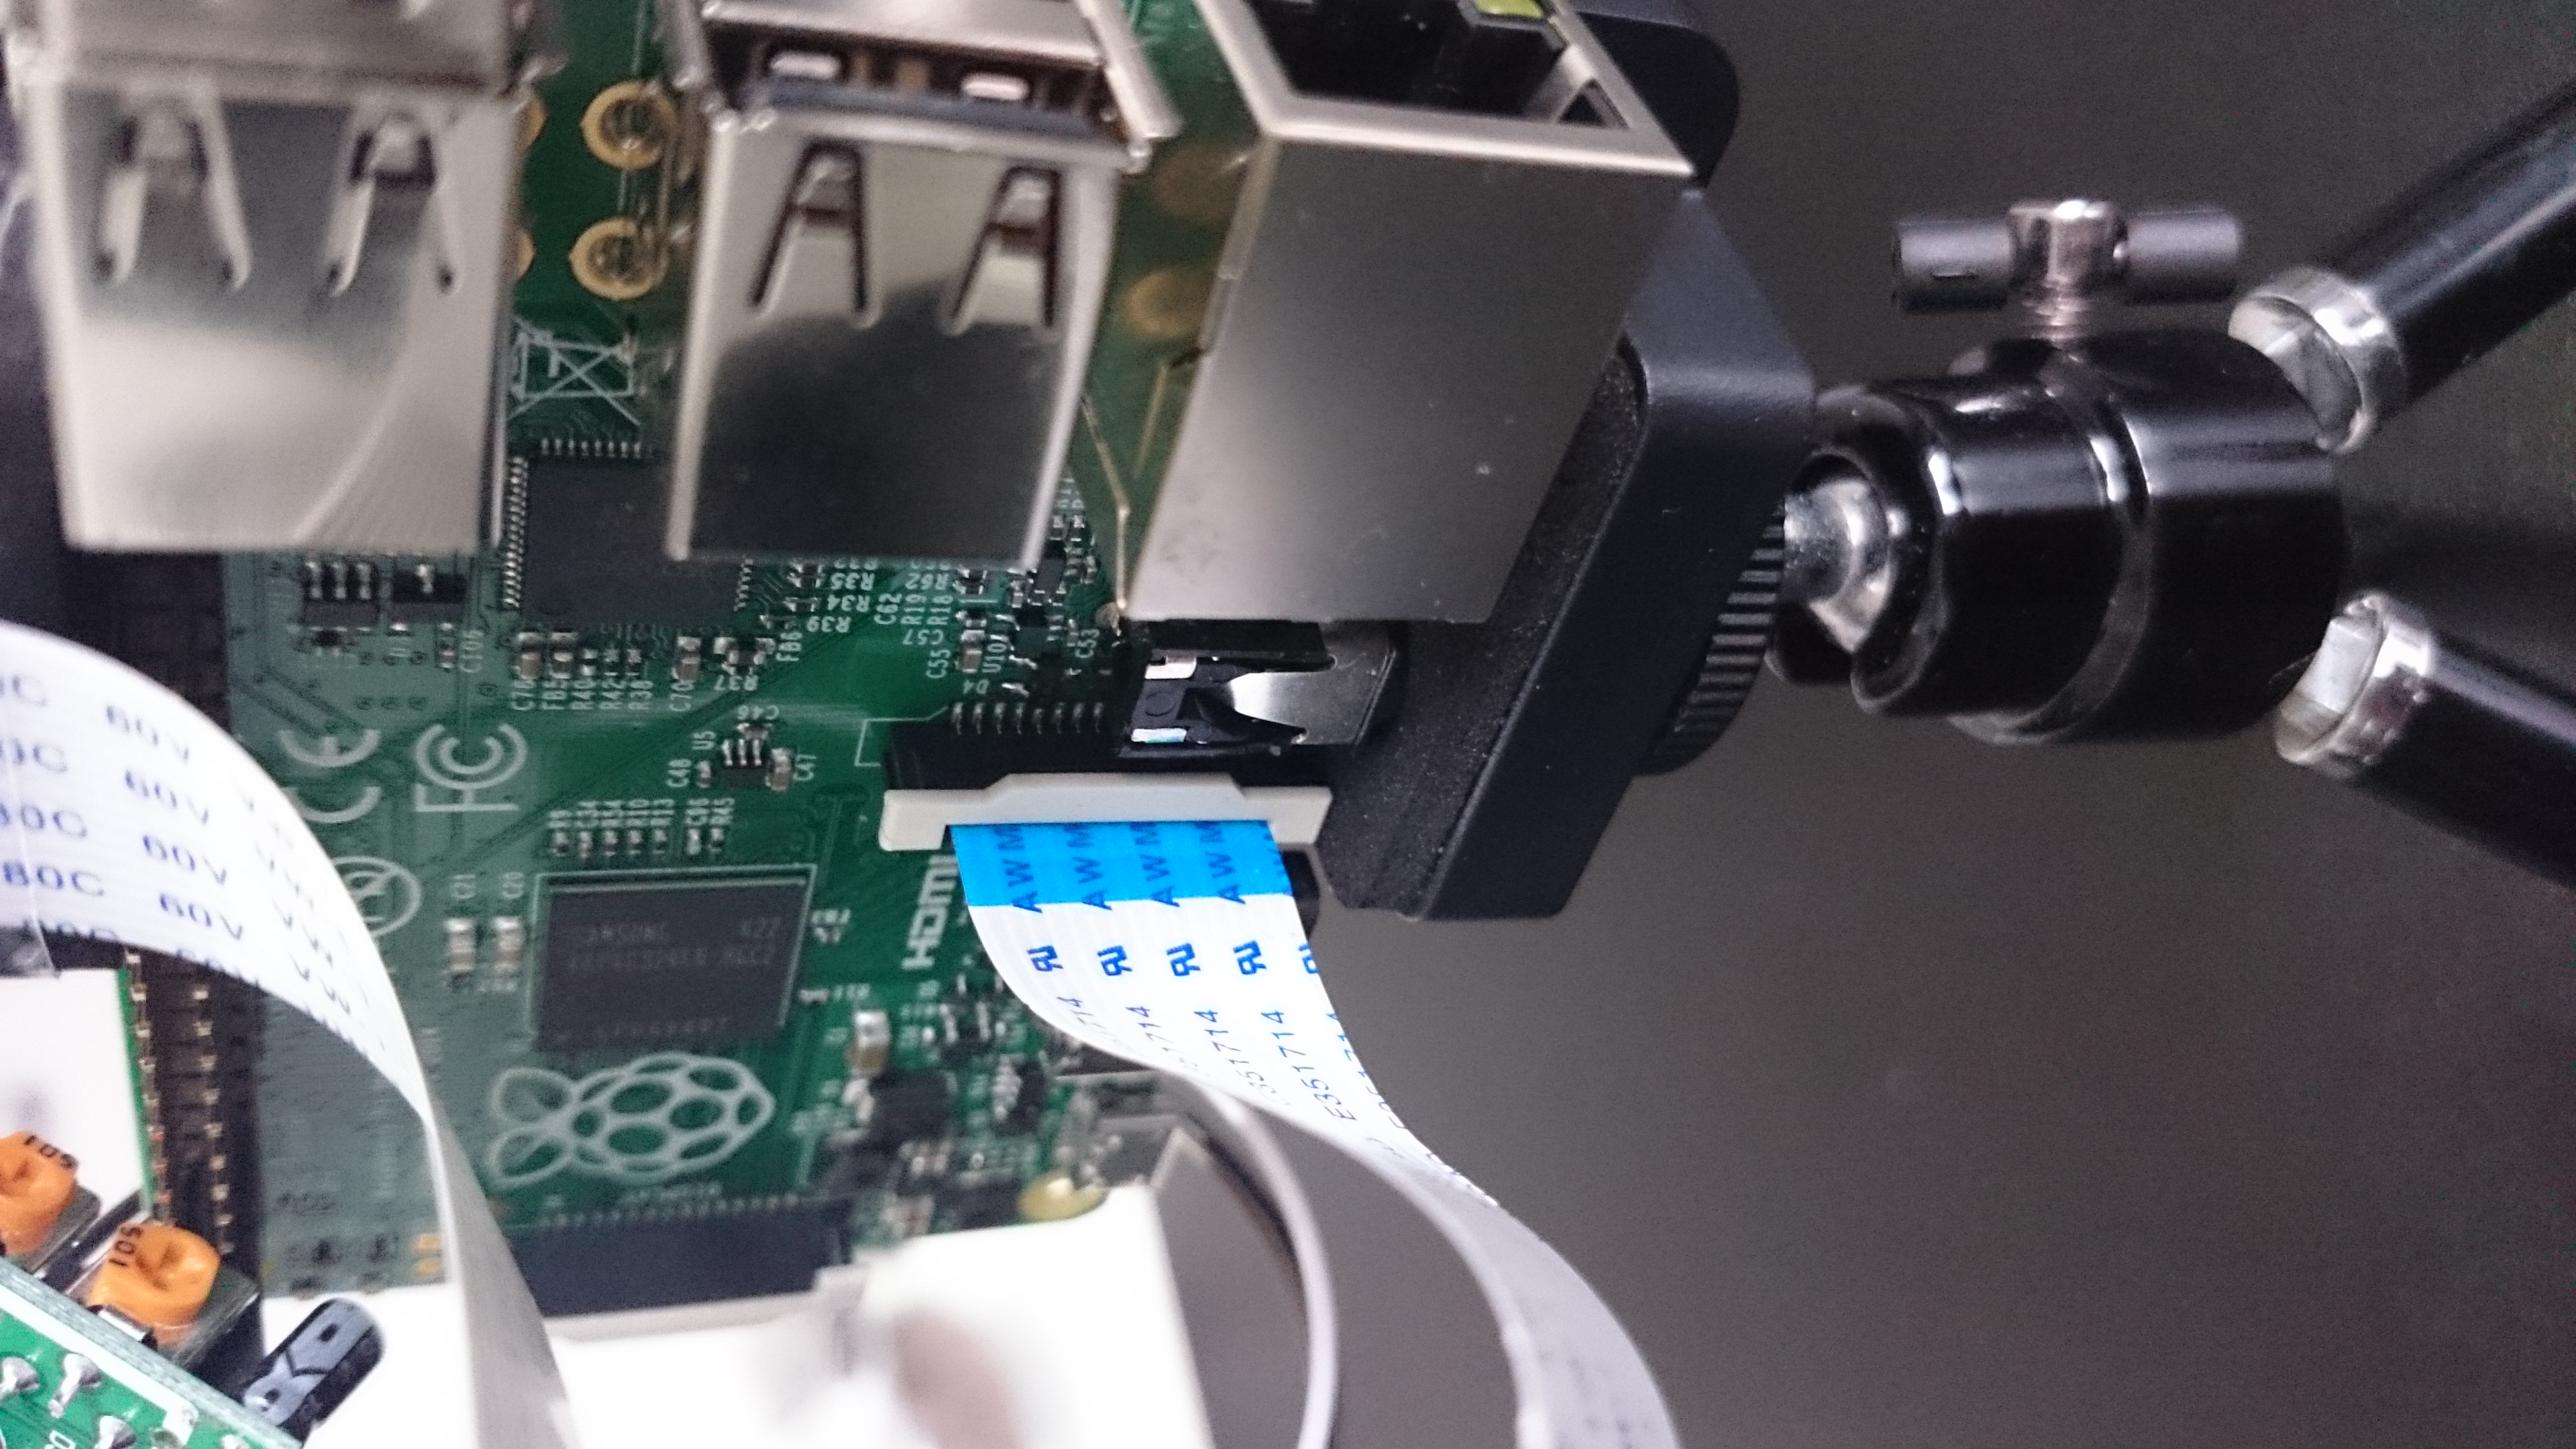
\includegraphics[width=7.9cm]{kamera.JPG} \caption{Anschluss für die Kamera} \end{figure}
Um die Kamera nutzen zu können, ist nicht viel Aufwand nötig. Schalten Sie den Raspberry Pi für die folgende Prozedur aus. Die Raspberry Pi Kamera wird mit einem Flachbandkabel ausgeliefert, für deren Anschluss nur eine einzige passende Schnittstelle zur Verfügung steht. Der Anschluss befindet sich vor dem LAN-Anschluss des Raspberry Pis. Das Flachbandkabel muss mit den Kontakten entgegengesetzt zum LAN-Anschluss eingesteckt werden. Wurde das Flachbandkabel eingesteckt, dann drücken Sie den Klemmverschluss runter, der das Flachbandkabel im Anschluss festhält. Starten Sie nun den Raspberry Pi und führen in der Kommandozeile den Befehl \textit{"sudo raspi-config"} aus. In diesem Menü gibt es für die Kamera einen eigenen Menüpunkt mit dem Namen: \textit{Enable Camera}.\begin{figure}[h] 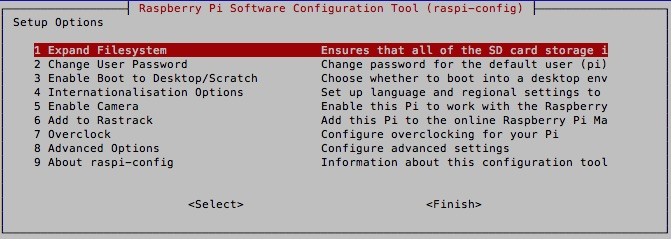
\includegraphics[width=15.8cm]{raspiconfig} \caption{Die Kamera wird unter Punkt 7 aktiviert} \end{figure} Wählen Sie diesen aus und bestätigen im nächsten Menü die Eingabe, indem Sie \textit{Enable} auswählen. Nach einem Neustart ist die Raspberry Pi Kamera auch schon einsatzbereit. Ob die Kamera auch richtig funktioniert, können Sie mit dem Befehl \textit{"raspivid -t 0"} testen (Achtung: Bild wird nur bei direkt angeschlossenem Monitor angezeigt). 

\section{Der PIR-Sensor}
Der PIR-Sensor muss, im Gegensatz zur Kamera, ohne eigens dafür vorgesehenen Anschluss auskommen. Hierfür müssen wir auf die Pins des GPIO-Boards auf dem Raspberry Pi zugreifen. Allerdings sollte auch hier der Anschluss nicht viel Zeit in Anspruch nehmen. Zunächst sollte für Arbeiten am GPIO-Board generell der Strom am Raspberry Pi abgeschaltet sein, um einen Kurzschluss zu vermeiden. Für den Anschluss empfiehlt es sich außerdem, eine durchnummerierte Übersicht über die einzelnen Pins des GPIO-Boards des Raspberry Pi zur Hand zu haben. Je nach Modell unterscheidet sich die Belegung und die Anzahl der einzelnen Pins. Auf der Seite des Raspberry Pi benötigen wir einen 3,3 Volt-Pin, einen GPIO-Pin und einen Ground-Pin. Bei allen Raspberry Pi Modellen müssen wir für den GPIO-Pin den Pin mit der Nummer sieben wählen. Unser Programm wird auf genau diesen Pin horchen und durch Signaländerungen auf diesem Pin beeinflusst. \begin{figure}[h] \centering 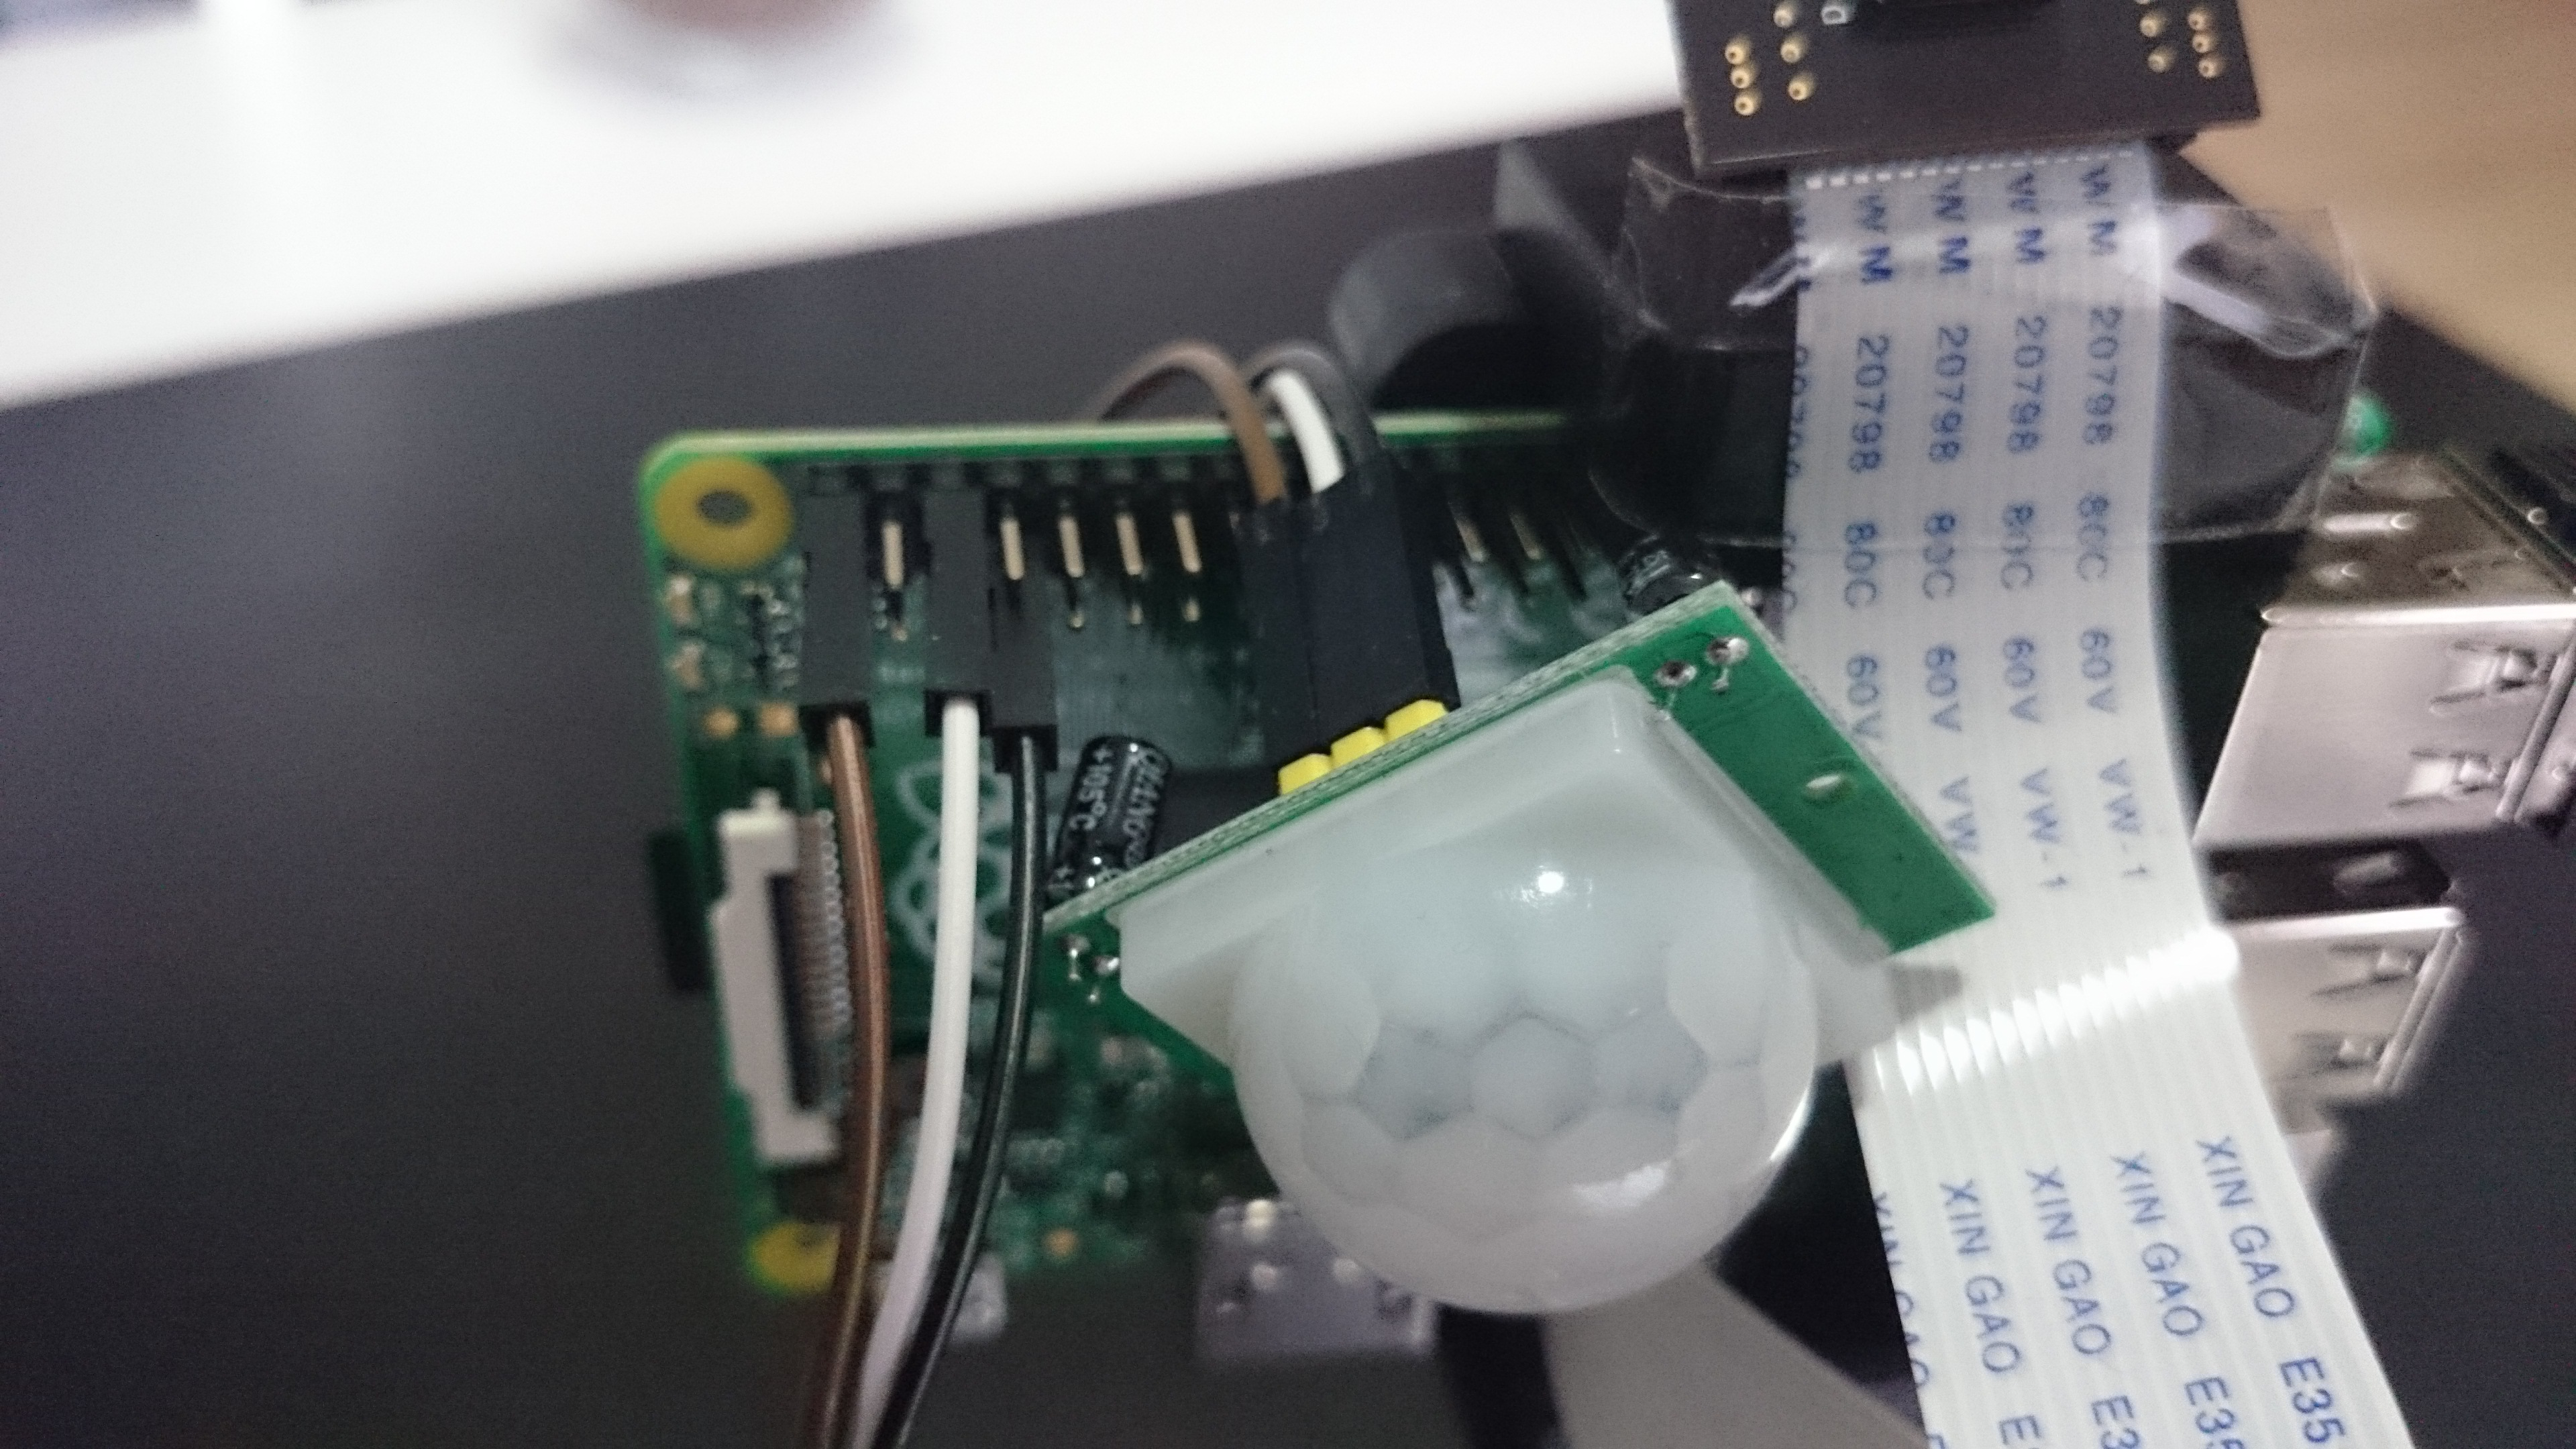
\includegraphics[width = 7.9cm]{pir1.JPG} \caption{Der fertig angeschlossene PIR-Sensor} \end{figure} \begin{figure}[h] \centering 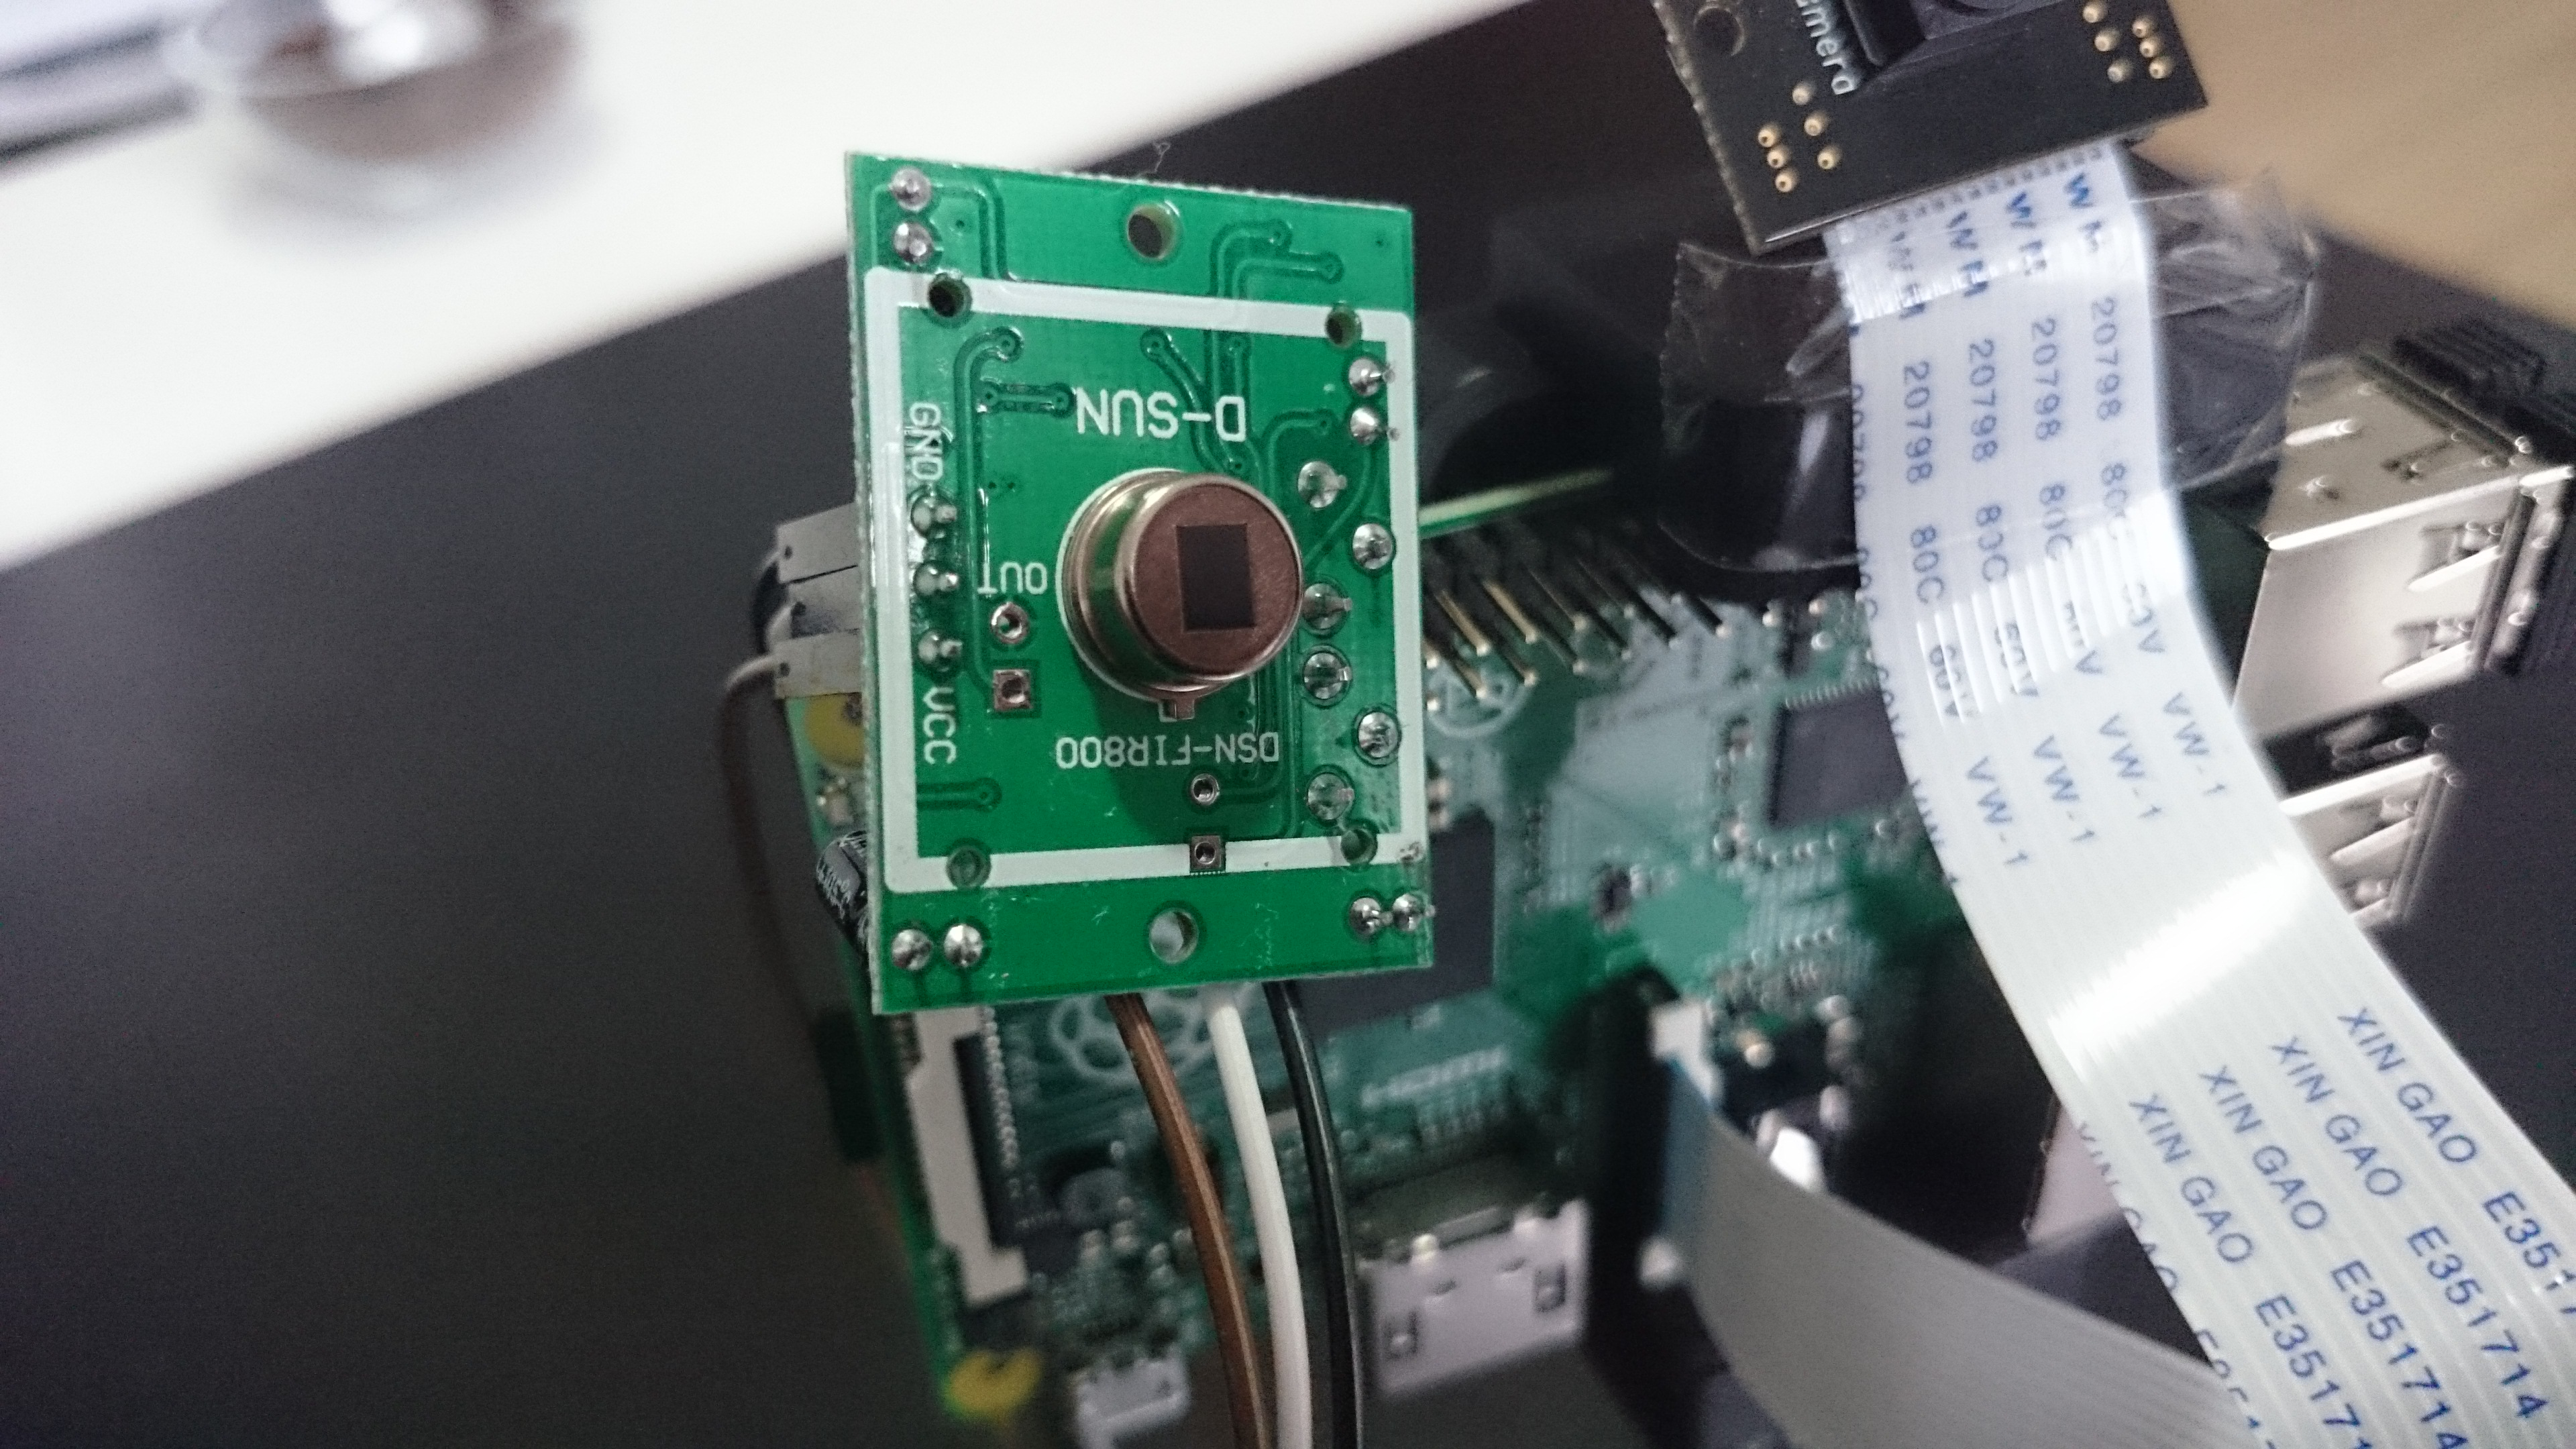
\includegraphics[width = 7.9cm]{pir2.JPG} \caption{Links sieht man gut die Beschriftung unter der Kuppel} \end{figure}Bei der Stromversorgung bleibt Ihnen die freie Wahl, wir schlagen allerdings Pin eins für die Stromversorgung mit 3,3 Volt und Pin sechs als Ground vor. Diese Konfiguration funktioniert auf allen Raspberry Pi Modellen. Um für den PIR-Sensor die jeweiligen Pins herauszufinden, müssen wir die milchige Kuppel auf dem Board des PIR-Sensors abziehen. Die Kuppel ist lediglich aufgesteckt und sollte leicht abzuziehen sein. Unter der Kuppel sehen wir, welcher Pin welchem Zweck dient. Stecken Sie nun die mit dem Raspberry Pi verbundenen Kabel auf ihre jeweiligen Gegenstücke auf dem Board des PIR-Sensors. Der Pin sechs vom GPIO-Board wird also auf den GND-Pin des PIR-Senors verbunden, Pin eins mit dem VCC-Pin des PIR-Sensors und Pin sieben mit dem mittleren OUT-Pin. Wenn Sie diese Schritte durchgeführt haben, können Sie den Raspberry Pi wieder mit dem Strom verbinden und hochfahren lassen. Ein Funktionstest ist jedoch nicht ohne Weiteres möglich, darauf müssen wir noch bis zur Inbetriebnahme der Software warten - oder Sie schreiben ein kleines Python-Script, dass die Funktion überprüft. Vergleichen Sie sonst Ihre Steckverbindungen mit der Abbildung 2.3.

\chapter{Das Programm}
\section{Codis einrichten und starten}
Sie können sich Codis aus folgendem Git-Repository besorgen: https://github.com/Lisiecki/codis.git
\\
Wir weisen darauf hin, dass in Zukunft Updates geplant sind, die Codis verbessern sollen bzw. einen Einsatz im Freien durch Bluetooth ermöglichen soll. Öffnen Sie nun, falls noch nicht geschehen, das Terminal und navigieren Sie in den Ordner, in welchem die Datei abgelegt wurde. Um das Programm zu starten, müssen Sie dieses mit dem Befehl \textit{"sudo python3 codis.py"} starten.\\ \textit{Wichtiger Hinweis:} Wenn Sie mehrere Raspberry Pis für Codis verwenden, achten Sie darauf Codis auf den einzelnen Raspberry Pis mit einem Mindestabstand von fünf Sekunden zu starten. Ansonsten kommt es zu Synchronisationsfehlern.\\

\section{Android-App um Signale zu empfagen}

Um überprüfen zu können, ob Codis einen Eindringling entdeckt hat, haben wir die sehr minimalistische Android-App Surveillance Receiver entwickelt. Diese App horcht auf den Port, den die Raspberry Pis im Codis-System verwenden, um miteinander zu kommunizieren und empfängt UDP-Pakete, die als Broadcast von den Raspberry Pis im Codis-System versendet werden. Die Surveillance Receiver App lässt sich aus dem selben Git-Repository runterladen, aus dem Sie bereits Codis runtergeladen haben: \textit{https://github.com/Lisiecki/codis.git}\\
Die Surveillance Receiver App unterstützt die Android-Versionen 4.1 bis 5.0.

\section{Funktionen der Surveillance Receiver App}

Im Folgendem erklären wir, was die Surveillance Receiver App kann. Auf dem Bildschirm wird ein prozentualer Wert dargestellt. Wird ein Eindringling entdeckt, wird vom Koordinator eine INTRUDER Nachricht versendet, die von der App empfangen wird. Empfängt die App die INTRUDER Nachricht, wird der Wert auf 100 Prozent gesetzt. Ist der Wert größer Null, werden jede Sekunde fünf Prozent vom Wert abgezogen. Empfängt die App wieder eine INTRUDER Nachricht, wird der Wert wieder auf 100 Prozent gesetzt. \\
Darüber hinaus befindet sich auf dem Bildschirm ein "Status"-Button. Wird der Button betätigt, geben alle Raspberry Pis im Codis-System ihren aktuellen Status im Terminal der jeweiligen Raspberry Pis zurück. Die Ausgabe beinhaltet die Position des Raspberry Pis in der Codis-Liste, die Größe der Codis-Liste, ob der Raspberry Pi der aktuelle Koordinator ist und ob der Raspberry Pi im Alarmzustand ist.


\end{document}